\chapter{Rappresentazione numeri frazionari con la virgola fissa}
\section{Idea}
Un sistema di numerazione in virgola fissa è quello in cui:
\begin{itemize}
    \item Si riserva un numero fisso di bit per parte intera e parte frazionaria
    \item La posizione della virgola decimale è implicita
    \item La posizione della virgola decimale è uguale in tutti i numeri
\end{itemize}

\section{UNSIGNED fixed point}
\subsection{Cosa è?}
La rappresentazione in virgola fissa non segnalata (Unsigned Fixec-Point) è una tecnica utilizzata per codificare e memorizzare numeri reali positivi (o nulli) all'interno di un numero finito di bit, mantenendo una posizione fissa per la virgola decimale

\subsection{Struttura del formato}
A differenza dei numeri interi, dove tutti i bit rappresentano potenze intere di 2, nella virgola fissa il totale di bit a disposizione($N$) viene suddiviso in 2 parti distinte da una posizione virtuale della virgola:
\begin{itemize}
    \item \textbf{Parte Intera ($I$ bit)}: Rappresenta la componente intera del numero
    \item \textbf{Parte frazionaria / decimale ($D$ bit)}: Rappresenta la parte dopo la virgola
\end{itemize}

Il totale dei bit sarà $N=I+D$, non essendo presente alcun bit per il segno, tutti i bit sono destinati al valore del numero

\begin{center}
    \begin{tabular}{|*{8}{c|}}
      \hline
      I-1 & I-2 & \dots & 0 & -1 & -2 & \dots & -D \\
      \hline
      \multicolumn{4}{|c|}{Parte Intera} & \multicolumn{4}{c|}{Parte Frazionaria} \\
      \hline
    \end{tabular}
\end{center}

\subsection{Range di valori rappresentabili}
\begin{itemize}
    \item Con questo metodo \textbf{l'intervallo di numeri interi} rappresentabili è: $[0,\ 2^{I-1}]$
    \item L'intervallo rappresentabile dalla \textbf{parte decimale} è $[0,\ 2^{D-1}]$
\end{itemize}

\newpage
\subsection{Peso delle posizioni}
Ogni bit ha un peso associato ad una potenza di 2, a seconda della sua posizione rispetto alla virgola:

{
    \large
    $$
    b_{I-1} \cdot \dots \cdot b_1 \cdot b_0 \cdot b_{-1} \cdot \dots \cdot b_{-D}
    $$
}

\begin{itemize}
    \item \textbf{Parte Intera}
    \begin{itemize}
        \item $b_0 \to 2^0 = 1$
        \item $b_1 \to 2^1 = 2$
        \item $b_0 \to 2^{I-1}$
    \end{itemize}
    \item \textbf{Parte Frazionaria}
    \begin{itemize}
        \item $b_{-1} \to 2^{-1} = 0.5$
        \item $b_{-2} \to 2^{-2} = 0.25$
        \item $b_{-3} \to 2^{-3} = 0.125$
        \item $b_{-D} \to 2^{-D}$
    \end{itemize}
\end{itemize}

Il valore decimale V corrispondente a una sequenza di bit si calcola sommando i pesi dei bit pari a 1:


{
    \LARGE
    $$
    \displaystyle V = \sum_{k=-D}^{I-1} b_k \cdot 2^k
    $$
}


\subsection{Da Decimale a Virgola Fissa Unsigned}
Prendiamo come esempio la conversione del numero decimale $23.625_{10}$ utilizzando un formato a 16 bit complessivi, con 8 bit per la parte intera ($I=8$) e 8 bit per la parte frazionaria ($D=8$)

\begin{enumerate}
    \item Si converte la parte intera in binario standard 
    {\large $$23_{10} = 16 + 4 + 2 + 1 = 2^4 + 2^2 + 2^1 + 2^0 = 0001\ 0111_{2}$$}
    
    \item Si moltiplica ripetutamente per 2 la parte frazionaria, prendendo la parte intera del risultato come bit e proseguendo con la nuova parte frazionaria fino a ottenere 0
    \begin{enumerate}
        \item $0.625 \times 2 = 1.25 \to 1$ (primo bit a destra della virgola)
        \item $0.25 \times 2 = 0.50 \to 0$ (secondo bit)
        \item $0.50 \times 2 = 1.00 \to 1$ (terzo bit, stop perchè la parte decimale è zero)
    \end{enumerate}
\end{enumerate}

Il risultato finale sarà:
\begin{itemize}
    \item $I = 0001\ 0111$
    \item $D = 101$
    \item Risultato finale = $0001\ 0111.10100000$
\end{itemize}

\subsection{Da Virgola Fissa Unsigned a Decimale}
Prendiamo la stringa binaria $$00010111.10100000_2$$ e calcoliamone il valore sommando i pesi delle posizioni con bit 1:

{
    \large
    $$\begin{aligned} V &= (1 \cdot 2^4) + (1 \cdot 2^2) + (1 \cdot 2^1) + (1 \cdot 2^0) + (1 \cdot 2^{-1}) + (1 \cdot 2^{-3}) \\ &= 16 + 4 + 2 + 1 + 0.5 + 0.125 \\ &= \mathbf{23.625_{10}}\end{aligned}$$
}

\newpage
\section{SIGNED fixed point}
\subsection{Struttura del formato}
L'unica differenza concettuale rispetto all'Unsigned è che il bit più significativo (MSB), ovvero il primo bit a sinistra, assume valore di peso pegativo

Data una lunghezza totale di $N = I + D$ bit:
\begin{itemize}
    \item 1 bit per il segno / parte intera più significativa
    \item $I-1$ bit per il resto della parte intera
    \item $D$ bit per la parte frazionaria
\end{itemize}

\subsection{Peso delle posizioni}

{
    \Large
    $$b_{I-1} \dots b_1 b_0 \,.\, b_{-1} b_{-2} \dots b_{-F}$$
}

\begin{itemize}
    \item \textbf{Bit di segno (MSB)}
    \begin{itemize}
        \item $b_{I-1} \to -2^{I-1}$
    \end{itemize}
    \item \textbf{Resto della parte intera}
    \begin{itemize}
        \item $b_1 \to 2^1 = 2$
        \item $b_0 \to 2^0 = 1$
    \end{itemize}
    \item \textbf{Parte Frazionaria}
    \begin{itemize}
        \item $b_{-1} \to 2^{-1} = 0.5$
        \item $b_{-2} \to 2^{-2} = 0.25$
        \item $b_{-D} \to 2^{-D}$
    \end{itemize}
\end{itemize}

Il valore decimale $V$ si calcola con la formula del complemento a 2 estesa ai decimali:

{
    \LARGE
    $$
    \displaystyle V = -b_{I-1} \cdot 2^{I-1} + \sum_{k=-D}^{I-2} b_k \cdot 2^k
    $$
}

\subsection{Da numero decimale positivo a Signed Fixed-Point}
I numeri positivi si codificano esattamente come nel caso unsigned, assicurandosi solo che il MSB sia 0

\begin{enumerate}
    \item \textbf{Parte intera}: $23_{10} = 0001\ 0111_{2}$
    \item \textbf{Parte frazionaria}: $0.625 \times 2 \dots \rightarrow .10100000_2$
    \item \textbf{Risultato}: ${00010111\,.\,10100000}_2$
\end{enumerate}

\newpage
\subsection{Da numero decimale negativo a Signed Fixed-Point}
Per codificare un numero negativo in CA2 a virgola fissa, il metodo semplice è complementare a 2 la rappresentazione del corrispondente numero positivo

\begin{enumerate}
    \item Prendi la stringa del valore positivo: $00010111.10100000$
    \item Invertire tutti i bit: $11101000.01011111$
    \item Aggiungi 1 al bit meno significativo (LSB), cioè all'ultimo bit della parte frazionaria:\\ $11101000.01011111 + 00000000.00000001$
    \item Risultato finale per $-23.625_{10}$: $\mathbf{11101000\,.\,01100000_2}$
\end{enumerate}

\chapter{Rappresentazionu numeri frazionari con la virgola mobile}

\section{Cosa è?}
La rappresentazione in virgola mobile è il metodo utilizzato dagli elaboratori per memorizzare e calcolare i numeri reali o numeri con ordini di grandezza estremamente grandi o piccoli.

\section{Struttura}
\subsection{32 bit}
I 32 bit totali sono suddivisi nel seguente modo:

\begin{center}
    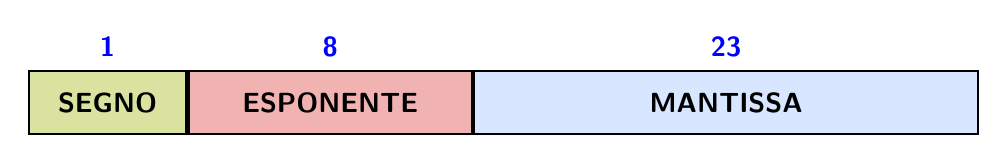
\begin{tikzpicture}[box/.style={draw=black, thick, minimum height=0.8cm, font=\bfseries\sffamily},
  num/.style={color=blue, font=\bfseries\sffamily, yshift=0.3cm}
    ]
    % Definizione colori locali
    \definecolor{colorSegno}{RGB}{218, 226, 160}
    \definecolor{colorEsponente}{RGB}{241, 178, 178}
    \definecolor{colorMantissa}{RGB}{216, 230, 255}

    % Blocchi
    \node[box, fill=colorSegno, minimum width=2.0cm] (segno) {SEGNO};
    \node[num] at (segno.north) {1};

    \node[box, fill=colorEsponente, minimum width=3.6cm, anchor=west] (esponente) at (segno.east) {ESPONENTE};
    \node[num] at (esponente.north) {8};

    \node[box, fill=colorMantissa, minimum width=6.4cm, anchor=west] (mantissa) at (esponente.east) {MANTISSA};
    \node[num] at (mantissa.north) {23};
    \end{tikzpicture}
\end{center}

\subsection{64 bit}
I 64 bit totali sono suddivisi nel seguente modo per la modalità a doppia precisione:
\begin{center}
        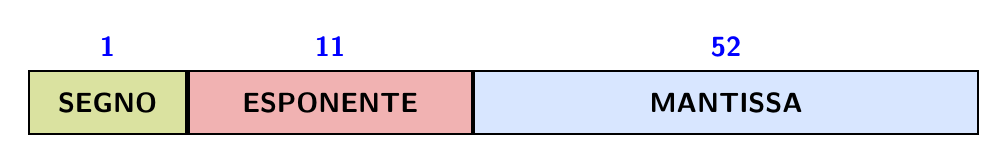
\begin{tikzpicture}[
    box/.style={draw=black, thick, minimum height=0.8cm, font=\bfseries\sffamily},
    num/.style={color=blue, font=\bfseries\sffamily, yshift=0.3cm}
    ]
    % Definizione colori
    \definecolor{colorSegno}{RGB}{218, 226, 160}
    \definecolor{colorEsponente}{RGB}{241, 178, 178}
    \definecolor{colorMantissa}{RGB}{216, 230, 255}

    % Blocchi del diagramma
    \node[box, fill=colorSegno, minimum width=2.0cm] (segno) {SEGNO};
    \node[num] at (segno.north) {1};

    \node[box, fill=colorEsponente, minimum width=3.6cm, anchor=west] (esponente) at (segno.east) {ESPONENTE};
    \node[num] at (esponente.north) {11};

    \node[box, fill=colorMantissa, minimum width=6.4cm, anchor=west] (mantissa) at (esponente.east) {MANTISSA};
    \node[num] at (mantissa.north) {52};
    \end{tikzpicture}
\end{center}

\section{Formule}
\subsection{Formula della rappresentazione in virgola mobile}
\begin{tcolorbox}
    {
        \LARGE
        $$
            N = (-1)^S \pm M \cdot B^{\pm E}
        $$
    }
    \begin{itemize}
        \item $S$ - Segno: Determina il segno del numero
        \item $M$ - Mantissa: È la parte frazionaria del numero. \\
        Contiene le cifre effettive del valore, di norma viene normalizzata
        \item $B$ - Base: È la base del sistema di numerazione utilizzato
        \item $E$ - Esponente: È l'esponente a cui viene elevata la base.\\
        Determina la posizione della virgola, ovvero l'ordine di grandezza del numero
    \end{itemize}
\end{tcolorbox}

\newpage
\subsection{Normalizzazione e "1 implicito"}
Per ottimizzare lo spazio di memoria, prima di codificare il numero in binario, lo si normalizza.

Un numero binario è formalizzato quando viene scritto nella forma

\begin{tcolorbox}
    {
        \LARGE
        $$
            \pm 1.M \cdot 2^E
        $$
    }    

    \begin{itemize}
        \item $M$ - Mantissa: È la parte frazionaria del numero. \\
        Contiene le cifre effettive del valore, di norma viene normalizzata
        \item $E$ - Esponente: È l'esponente a cui viene elevata la base.\\
        Determina la posizione della virgola, ovvero l'ordine di grandezza del numero
    \end{itemize}
\end{tcolorbox}

\section{Conversione da Decimale a Virgola Mobile}

Convertiamo il numero 13.25 in virgola mobile a 32 bit

\begin{enumerate}
    \item \textbf{Determinare il segno}: Il numero è positivo, quindi il bit del segno ($S$) è 0
    \item \textbf{Convertire la parte intera e frazionaria in binario}
    \begin{enumerate}
        \item \textbf{Parte intera}: 31 = 1101
        \item \textbf{Parte frazionaria}: Si moltiplica ripetutamente per 2 la parte decimale:
        \begin{enumerate}
            \item $0.25 \cdot 2 = 0.5 \to 0$
            \item $0.50 \cdot 2 = 1.0 \to 1$
        \end{enumerate}
    \end{enumerate}
    Otteniamo la forma binaria: $1101.01_2$

        \item \textbf{Normalizzare il valore}: Spostiamo la virgola a sinistra di 3 posizioni per ottenere la forma $1.xxx$

        $$
            1101.01_2 = 1.10101_2 \cdot 2^3
        $$

        \begin{itemize}
            \item L'esponente reale (E) è 3
            \item La parte a destra della virgola (Mantissa - M) è 10101
        \end{itemize}

    \item \textbf{Calcolare l'esponente in Eccesso 127}: Aggiungiamo la costante di offset all'esponente reale

    $$
        E = 3 + 127 = 130_10
    $$
    
    Convertendo 130 su 8 bit in binario otteniamo: 10000010

    \item \textbf{Assemblare la sequenza di 32 bit}
    \begin{itemize}
        \item Segno (1 bit) = 0
        \item Esponente (8 bit) = 10000010
        \item Mantissa (23 bit) = 10101 allungato con zeri a destra fino a completare i 23 bit: 
        
        10101000000000000000000
    \end{itemize}
    Risultato finale:
    $$
        0\ 10000010\ 10101000000000000000000     
    $$
\end{enumerate}

\section{Conversione da Virgola Mobile a Decimale}
Data la sequenza $1\ 10000000\ 11000000000000000000000$

\begin{enumerate}
    \item \textbf{Segno}: Il primo bit è 1, dunque il numero è negativo
    \item \textbf{Esponente}: $$10000000_2 = 128_{10}$$

    Sottraendo l'offset 127: $e = 128 - 127 = 1$
    
    \item \textbf{Mantissa}: 11000000000000000000000 rappresenta 
    $$2^{-1} + 2^{-2} = 0.5 + 0.25 = 0.75$$

    \item \textbf{Ricostruzione del valore}
        $$
        \text{Valore} = - (1 + \text{Mantissa}) \times 2^e = - (1 + 0.75) \times 2^1 = -1.75 \times 2 = -3.5_{10}
        $$
\end{enumerate}

\section{Errore assoluto $E_a$}
\subsection{Cosa è?}
L'errore assoluto indica la differenza diretta tra il valore reale esatto e il valore approssimato memorizzato.

Rappresenta lo scarto fisico o la distanza quantitativa tra la misura reale e quella approssimata, mantenendo la stessa unità di misura del dato di partenza

\subsection{Formula}

\begin{tcolorbox}
    {
        \LARGE
        $$
            E_a = \vert{}V - \tilde{V}\vert{}
        $$
    }

    \begin{itemize}
        \item $V$: Valore realae
        \item $\tilde{V}$: Valore approssimato memorizzato
    \end{itemize}
\end{tcolorbox}

\subsection{Esempio di calcolo}

\subsubsection{Dati di partenza}
Ipotizziamo di dover rappresentare una grandezza fisica o un numero reale in un calcolatore:

\begin{itemize}
    \item \textbf{Valore reale esatto ($V$)}: $14.888$
    \item \textbf{Valore approssimante memorizzato ($\tilde{V}$)}: $14.900$
\end{itemize}

\subsubsection{Calcolo}
{
    \Large

    $$
    E_a = \vert{} 14.888 - 14.9000 \vert{} = \vert{} -0.012 \vert{} = 0.012
    $$
}

\section{Errore Relativo $E_r$}
\subsection{Cos'è?}
L'errore relativo misura l'incidenza dell'errore assoluto rispoetto alla grandezza del numero di partenza.

Un errore assoluto di 0.1 è enorme se si sta misurando un oggetto lungo1, ma è del tutto trascurabile se si sta misurando una distanza di 1000000.

Per questo motivo, l'errore relativo è un numero adimensionale ed è fondamentale per valutare la precisione di una rappresentazione

\subsection{Formula}

\begin{tcolorbox}
    {
        \Large

        $$
            E_r = \frac{E_a}{|V|} = \frac{|V - \tilde{V}|}{|V|}
        $$
    }

    \begin{itemize}
        \item $E_a$: Errore assoluto
        \item $V$: Valore realae
        \item $\tilde{V}$: Valore approssimato memorizzato
    \end{itemize}
\end{tcolorbox}

\subsection{Esempio di calcolo}
Supponiamo di voler rappresentare il valore reale $V = 14.888$ tramite un numero discreto con un passo di discretizzazione, dove il valore approssimante più vicino è $\tilde{V} = 14.9$:

\begin{enumerate}
    \item \textbf{Calcolo dell'errore assoluto}
    $$
        E_a = |14.888 - 14.9| = |-0.012| = 0.012
    $$
    \item \textbf{Calcolo dell'errore relativo}
    $$
        E_r = \frac{0.012}{14.888} \approx 0.00080602
    $$
    \item \textbf{Calcolo dell'errore relativo percentuale}
    $$E_r\% = 0.00080602 \times 100\% \approx 0.0806\%$$
\end{enumerate}